\documentclass[11pt]{article}

\usepackage{geometry}


\usepackage[T1]{fontenc}
\usepackage{longtable,amsmath,tabularx}
\usepackage{bigfoot} % to allow verbatim in footnote
\usepackage[numbered,framed]{matlab-prettifier}
\usepackage{array}
\usepackage{booktabs}
\usepackage{graphicx}
\usepackage{amsmath}

\usepackage{subfiles}

\usepackage[hidelinks]{hyperref}
\hypersetup{
	colorlinks=false, %set true if you want colored links
	linktoc=all,
}

	\newgeometry{
	a4paper,
	left=25mm,
	right=25mm,
	top=25mm,
	bottom=25mm,
}

\usepackage[toc,page]{appendix}

\usepackage{lscape}

\usepackage{float}

\usepackage{times}

\usepackage{caption} 
\captionsetup[table]{skip=10pt}

\usepackage{tikz}

\fontfamily{ptm}\selectfont

\lstset{
	style              = Matlab-editor,
	basicstyle         = \mlttfamily,
	escapechar         = ",
	mlshowsectionrules = true,
}


\usepackage{fancyhdr}

\pagestyle{fancy}
\fancyhf{}
\rhead{CP3403}
\lhead{Data Mining Project}
\rfoot{Page \thepage}

\begin{document}
	
	\begin{titlepage}
		\begin{center}
			\vspace*{1cm}
			
			\Huge
			\textbf{Classifying Hand Gestures from EMG Data}
			
			\vspace{0.5cm}
			\LARGE
			CP3403 - Data Mining Project
			
			\vspace{1.5cm}
			
			\textbf{Joshua Gray - 13177877}\\	
			\textbf{Harmon Singh - }
			
			\vfill			
					
			\vspace{0.8cm}
			
			
\includegraphics[width=0.4\textwidth]{Figures/jculogo}
			
			\Large
			College of Business, Law and Governance\\
			James Cook University\\
			Australia\\
			25/05/2019
			
		\end{center}
	\end{titlepage}
	
	\pagenumbering{roman}
	\tableofcontents
	\listoffigures
	\listoftables
	\newpage
	\pagenumbering{arabic}
	
	\section{Introduction}
	Since the turn of the 20th century, a lot of focus has been placed on the incorporation and integration of technology in medical fields. This relationship between medicine and technology has spawned a multitude of life-saving devices such as the Automated External Defibrillator and non-invasive diagnostic tools such as Magnetic Resonance Imaging and Computed Tomography.\\
	
	\noindent	
	With the widespread increase of data mining and analysis in recent years as well as vast improvements in computing and storage power available today, a logical question for the data science community is finding the ways in which this area has the potential of improving the medical industry. In addition to this, in what way can the Internet of Things enable this kind of technology? A field which has attempted to improve the quality of life for it's patients since the beginning is the field of prosthetics.\\
	
	\noindent
	
	
	\section{Artificial Neural Networks}
	The field of classification has been plagued in recent years by the popularity of the Artificial Neural Network (ANN). Constantly evolving, ANN's are machine learning systems that aim to simulate the functionality of biological networks such as the human brain. As they have a constant defined structure, they excel when compared to some other methods as they have no bias from the programmer i.e. they are defined generally, with the data forcing biases in the output of the system.\\
	
	\noindent
	The basic functionality of ANN's remain the same between different implementations. The building block of all neural networks is the implementation of the "neuron". A neuron is modelled as a weighted function of its inputs. As given by Figure \ref{fig:neuron}, the inputs $x_i$ are weighted by a factor $w_i$ with an added bias $b$. All of these inputs are then summed and passed through an activation function $f_a$ which filters the output $y$.\\
	
	\begin{figure}[H]
		\centering
		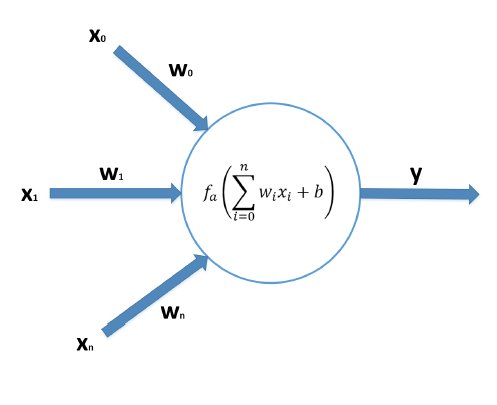
\includegraphics[width=10cm]{Figures/neuron}
		\caption{Simple ANN Neuron}\cite{Bonaccorso2017}
		\label{fig:neuron}
	\end{figure}

	\subsection{Multi-layer Perceptron}
	With this simple neuron functionality, the implementation of the Multi-layer Perceptron (MLP) system can be realises. An MLP system consists of fully connected "layers" of neurons. At their most simple level, they can be realised with a minimum of three layers. The first layer, the input layer is the place in which raw information enters the network. This layer is un-weighted and each neuron fully connects to the next layer, the "hidden" layer. The hidden layer can be a single layer and up to as many layers as the developer chooses. These layers are fully connected i.e. each output connects to every neuron in the next layer. The final layer is called the output layer. This layer is the direct point in which interfacing with the neural network is performed. Depending on the task required, the function of the output layer may vary. The implementation of MLP for this project is explored in Section \ref{sec:mlp_class}.
	
	\begin{figure}[H]
		\centering
		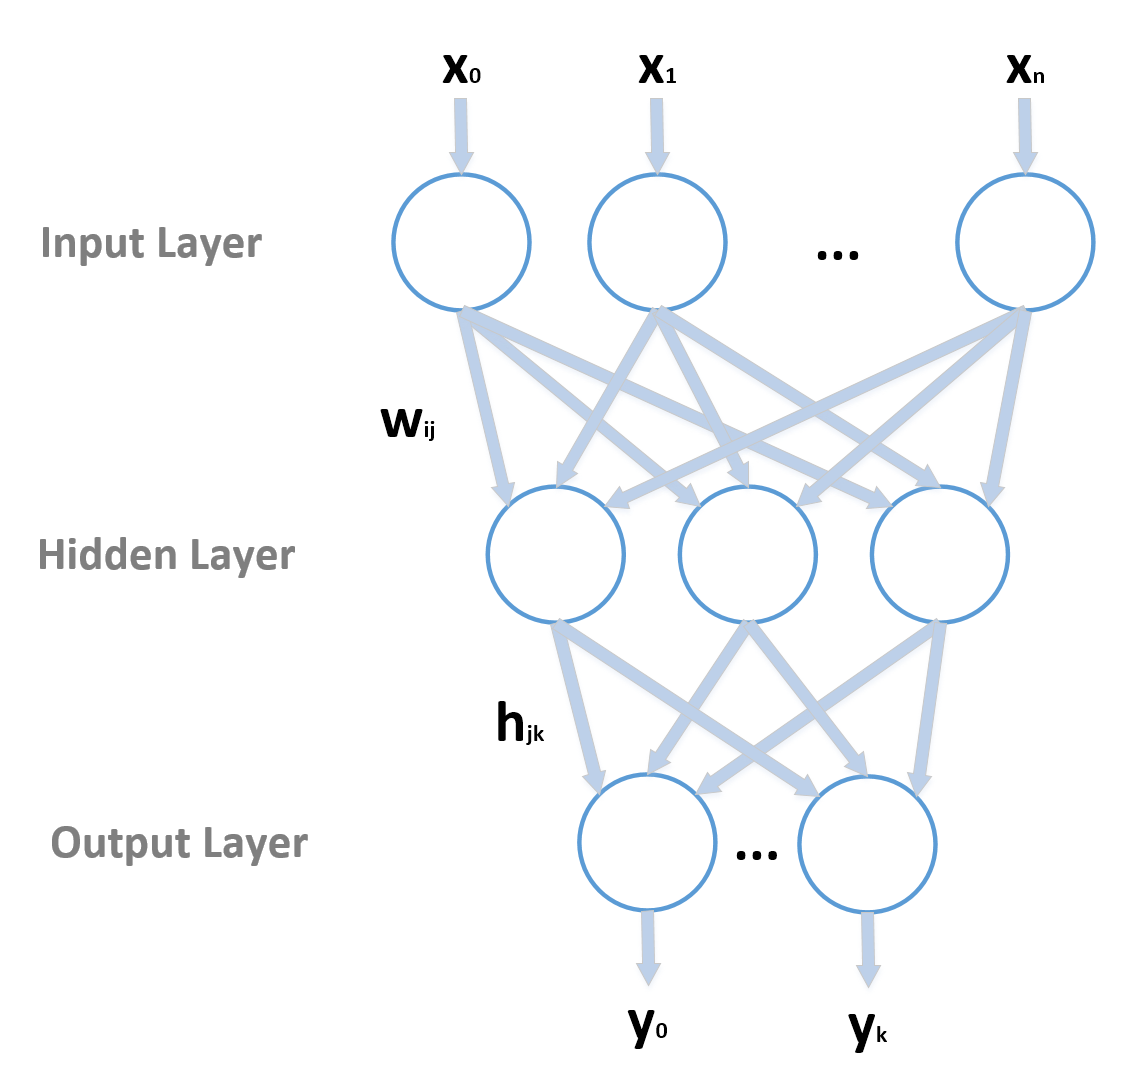
\includegraphics[width=10cm]{Figures/mlp}
		\caption{Simple MLP Network}\cite{Bonaccorso2017}
		\label{fig:mlp}
	\end{figure}
	
	\subsection{MLP's and Classification}\label{sec:mlp_class}
	
	
	\section{EMG Data for Gestures Data Set}
	The EMG Data for Gestures Data Set (Available from: \url{https://archive.ics.uci.edu/ml/datasets/EMG+data+for+gestures}) was a data set created for determining latent factors in the performance of sEMG interfaces \cite{Lobov2018}. The overall achievement of this paper was identifying some potential medical influences on the use of EMG interfaces to measure gesture information.\\
	
	\noindent
	This particular dataset was obtained through the use of the Myo Thalmic bracelet (See Figure \ref{fig:myo}). The EMG channel recordings were obtained through a Bluetooth interface to a computer. A total of eight channels are recorded with each of the sensors equally spaced around the forearm of the subjects recorded.\\
	
	\begin{table}[H]
		\caption{Attributes of the Raw Data Set}
		\centering
		\begin{tabular}{l|l}
			Attribute   & Description             \\\hline
			Time        & Time Step of  Recording (Numeric)\\
			Channel 1-8 & Raw EMG Measurement (Double Precision Float)     \\
			Class       & Gesture Performed (Numeric 0-7)      \\\hline\hline
		\end{tabular}
	\end{table}

\begin{table}[H]
	\caption{Descriptions of Attribute Class}
	\centering
	\begin{tabular}{l|l}
		Class & Description             \\\hline
		0     & Unassigned              \\
		1     & Hand at rest            \\
		2     & Hand clenched in a fist \\
		3     & Wrist Flexion           \\
		4     & Wrist Extension         \\
		5     & Radial Deviations       \\
		6     & Ulnar Deviations        \\
		7     & Extended Palm           \\\hline\hline
	\end{tabular}
\end{table}
	
	\noindent
	A total of 36 subjects were used for this experiment. Each subject performed a series of static hand gestures (a total of 7 unique gestures) with a 3 second gap between the recording of each gesture. The series were also repeated twice for each subject.\\
	
	\noindent
	The values recorded by each channel are represented in scientific format corresponding to a double precision floating point number. The magnitude corresponds to the potential measured by the device at the skin level but units were withheld from the data. Further information about the Myo armband revealed that raw EMG data should be transferred as uint8 values corresponding to the amount of "activation" of the muscle \cite{myo_data} but this is not reflected in the data. Based on preliminary analysis, the data should be sufficient as the final system should adapt to incoming signals without the need of specific input data (As long as the format is known). \\
	
	\noindent
	An important thing to note for this data set is that due to the nature of the data (different subjects), the general classification task will prove more difficult as there are physiological aspects that affect the magnitude of the readings. As explored in \cite{Lobov2018}, people who have greater muscle development in their forearms generally show higher magnitudes on the EMG readings and people with higher body fat content generally have smaller magnitudes.
	
	\begin{figure}[H]
		\centering
		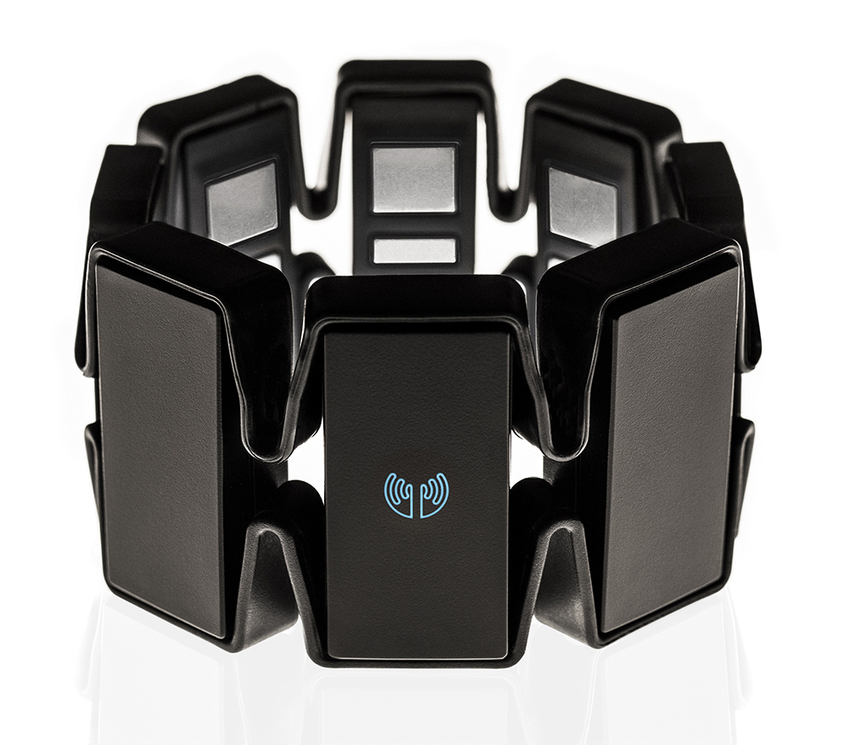
\includegraphics[width=10cm]{Figures/myo_armband}
		\caption{Thalmic Labs Myo Bracelet}
		\label{fig:myo}
	\end{figure}

	\noindent
	Due to the discontinuation of the Myo armband in 2018, this dataset is unlikely to be able to be replicated or in future. However, the design of the final analysis system should be independent of the recording device used (as preprocessing should solve this problem). As is the design of many systems in use today, modularity is key for these devices to remain cost effective for the end users. 
	
	\section{Preprocessing}
	Preprocessing is a crucial step of any data analysis task. Much like any other analysis, the quality of the outputs of the system is directly dependent on the quality and accuracy of the inputs. In addition to this, deeper knowledge of the system is also useful in mapping input data values into system values.\\
	
	\noindent
	For this system, the following is known about the nature of the data:
	
	\begin{itemize}
		\item \textbf{Values - } The values recorded in the data can generally be represented in scientific notation with up to 5 decimal places. 
		\item \textbf{Data Nature - } According to the data sets provided information\cite{Lobov2018}, the data recorded are raw EMG values measured by the Myo armband. As such, special treatment of these values is required to  generate reasonable predictions.
		\item \textbf{Data Bias - } As 36 subjects were used to conduct this experiment and the overall goal of this system is to generalise a system for classification, special consideration was required to obtain an accurate representation of the whole data set.
	\end{itemize}

	\noindent
	With these goals in mind, a system was designed to both format and clean data as well as prepare it for an MLP system. To design the system the most efficiently and allowing the ability for further experimentation, the system was to be designed in two steps. The first step was the formatting and cleaning of the data files into a format that could be directly imported into a Relational Database Management System (RDBMS). The second section was then the direct mapping of values into a format conducive to making classifications by the MLP system. 
	
	\subsection{Data Format Tool} \label{sec:data_format}
	The first section of the overall preprocessing system was to develop a system to interface between raw data values and the RDBMS system storing all the training data for this project. For the sake of reproducibility, this section was designed to interface directly with the EMG Data for Gestures Data Set. Although a reasonably trivial process, it was important to structure the output data in such a way that all systems are able to interpret. The following flow chart describes the functionality of this section.	\\
	\begin{figure}[H]
		\centering
		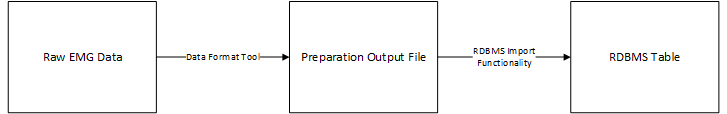
\includegraphics[width=15cm]{Figures/format_system}
		\caption{Data Flow of the Formatting System}
		\label{fig:data_format}
	\end{figure}

	\noindent
	Table \ref{tbl:histo} show the distribution of values across each channel. This table was created using the popular data-mining tool WEKA. Due to the size of the input values and the implementation of the WEKA interface, little data insights are directly available. However, the distribution of values for the raw data indicate that there is a fair chance that the data is relatively clean with small quantities of outliers and a very defined bell curve shape about the resting value (channel reading 0). 

	\begin{table}[H]
		\centering		
		\caption{Histogram of values across the EMG Data for Gestures Data Set}
		\label{tbl:histo}
		\begin{tabular}{cc}
			\toprule
			Channel & Histogram\\
			\midrule
			1 & 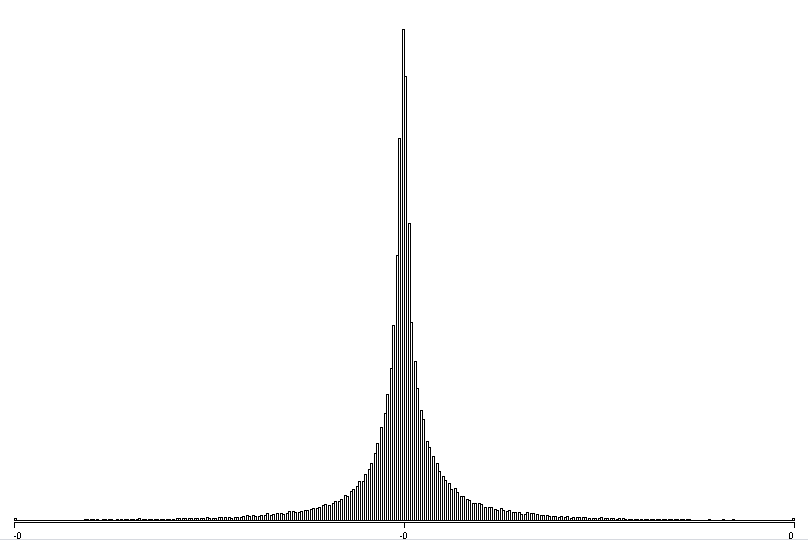
\includegraphics[height=2.5cm, width=12cm]{Figures/Stats/channel1}\\
			2 & 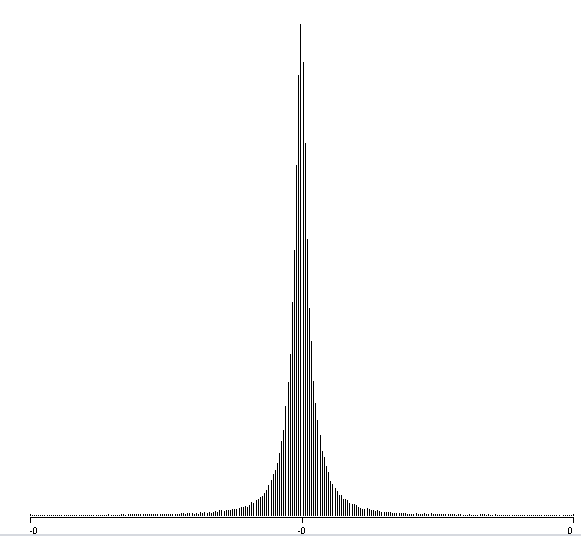
\includegraphics[height=2.5cm, width=12cm]{Figures/Stats/channel2}\\
			3 & 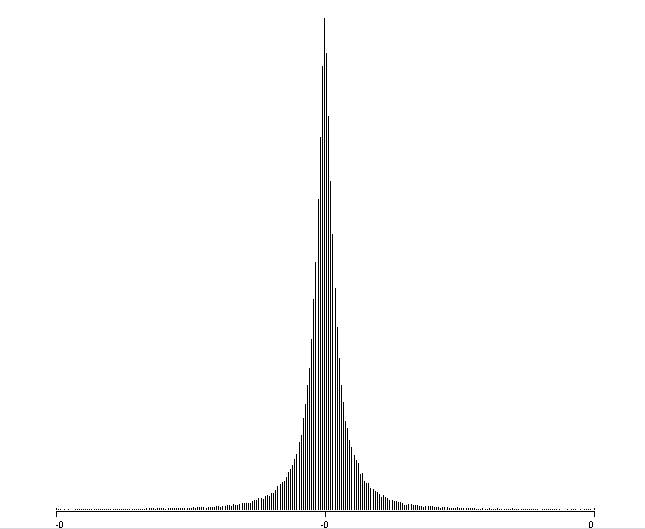
\includegraphics[height=2.5cm, width=12cm]{Figures/Stats/channel3}\\
			4 & 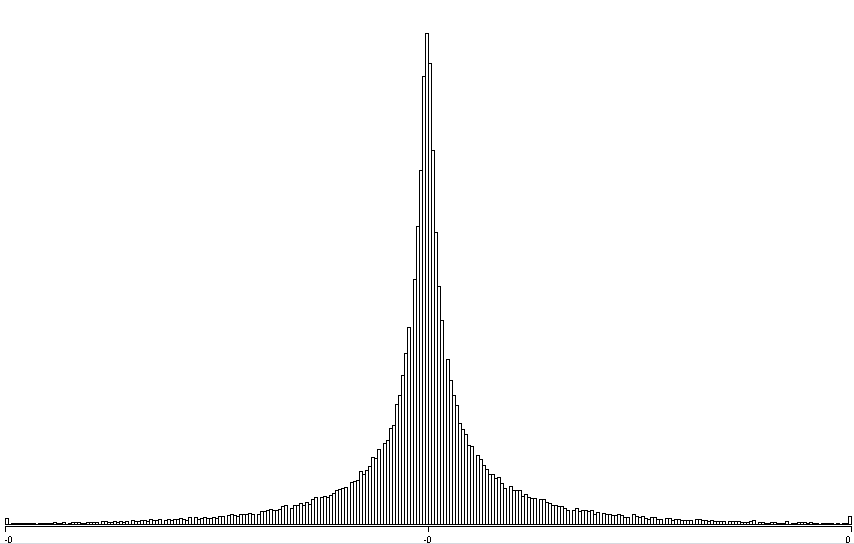
\includegraphics[height=2.5cm, width=12cm]{Figures/Stats/channel4}\\
			5 & 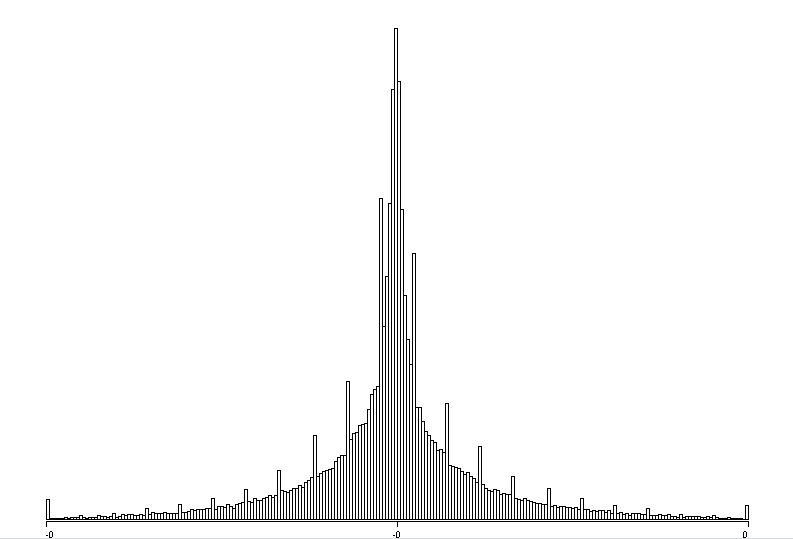
\includegraphics[height=2.5cm, width=12cm]{Figures/Stats/channel5}\\
			6 & 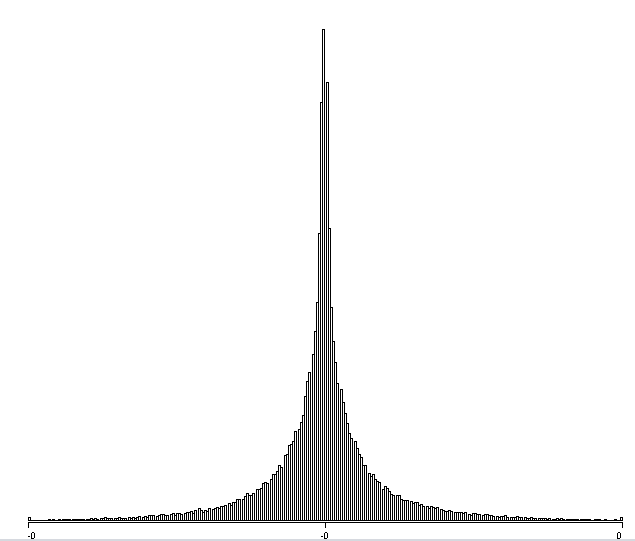
\includegraphics[height=2.5cm, width=12cm]{Figures/Stats/channel6}\\
			7 & 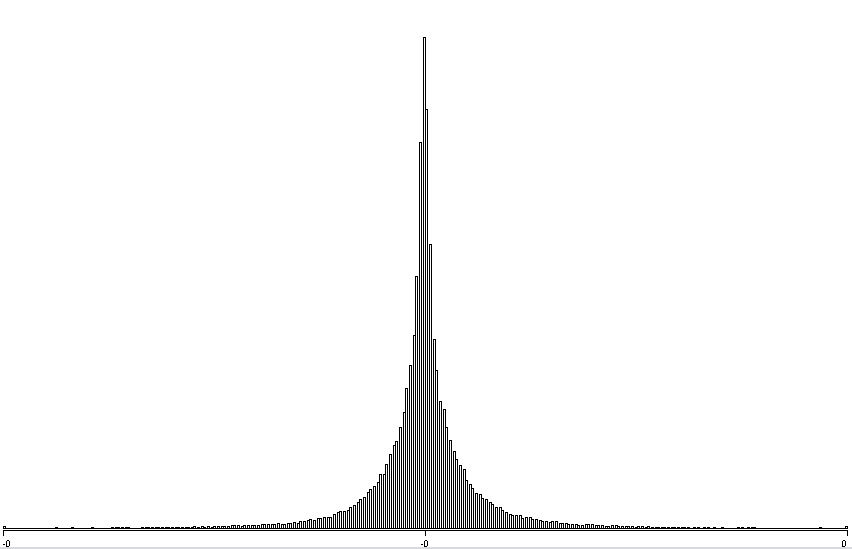
\includegraphics[height=2.5cm, width=12cm]{Figures/Stats/channel7}\\
			8 & 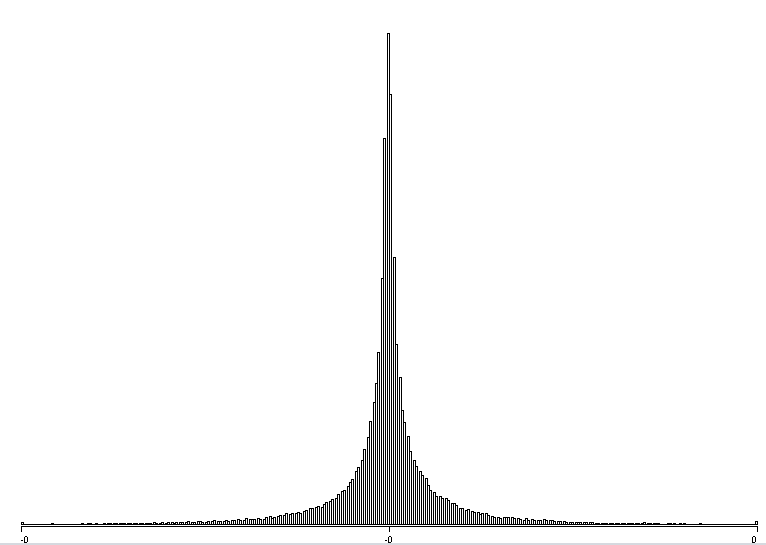
\includegraphics[height=2.5cm, width=12cm]{Figures/Stats/channel8}\\
			\bottomrule
		\end{tabular}
	\end{table}

	\noindent
	The original data file structure consists of multiple folders relating to each subject with multiple data files for each test performed. The data format module was designed such that the entire file-system will be traversed and each file available on the system is read and converted into the desired interim format. The full exploration of the data format module can be seen in Appendix  \ref{adx:data_format}. Beyond this, the data format tool has the following features
	
	\begin{itemize}
		\item Unmarked data is completely removed
		\item Incomplete data is ignored
		\item Records are randomised at the conclusion of the import (Generalising the data)
		\item Records are outputted to a single csv file that is directly importable into SQL Server
	\end{itemize}

	\subsection{Data Storage}
	Data storage for this task is an important one, With hundreds of thousands of records available, it is important to develop a system for access and storage of this information. Being a staple of the business world for the last few decades, SQL is an appropriate choice for this task. For this project, Microsoft SQL Server Professional 2017 was chosen as the RDBMS for the gestures data. The output of the Data format tool explained in Section \ref{sec:data_format} can be directly imported into SQL Server through the use of Microsoft's SQL Server Import and Export Wizard. 
	
	\begin{table}[H]
		\centering
		\caption{Gestures Table Structure in SQL Server}
		\begin{tabular}{l|llll}\hline	
			Field    & Data Type & Data Length & Precision & Primary Key \\\hline
			record   & int       & 4           & 10        & 1           \\
			channel1 & float     & 8           & 53        & 0           \\
			channel2 & float     & 8           & 53        & 0           \\
			channel3 & float     & 8           & 53        & 0           \\
			channel4 & float     & 8           & 53        & 0           \\
			channel5 & float     & 8           & 53        & 0           \\
			channel6 & float     & 8           & 53        & 0           \\
			channel7 & float     & 8           & 53        & 0           \\
			channel8 & float     & 8           & 53        & 0           \\
			class    & int       & 4           & 10        & 0           \\\hline\hline
		\end{tabular}
	\end{table}

	\noindent
	The last aspect of the data storage system is accessing the data within the MLP software. This is done using an ODBC driver written in python (pyodbc). Being a generic driver for database connectivity, this interface should be accessible for different RDBMS software (Oracle or MySQL) as well as different programming languages as the ODBC driver is implemented in all major programming languages.

	\subsection{Data Processing}
	Much unlike many problems in Data Mining, the preprocessing for this system lies primarily in the ability to use insights of the raw data in order to process them for a neural network. As it is inherently a signal processing problem\cite{emg_analysis}, the following is assumed of the Gestures data based on the range of values:
	
	\begin{itemize}
		\item DC offset is removed from the signal
		\item The signal has been applied with low-pass filtering before recording
		\item Presence of negative values eludes to rectification and time-averaging not being performed on the data. This may be a serious issue as theoretically, the values recorded might not be time-representative of the gesture.
	\end{itemize}

	\noindent
	Based on this, the first step of data processing is to "rectify" the incoming values. As the EMG data is an electrical signal based on activity produced by skeletal muscles, the value of such signal are sinusoidal in nature. Given this, the sign of record values is irrelevant to the classification task and in order to minimise confusion of the MLP system, were removed.\\
	
	\noindent
	The next step is to prepare the values to be used with the chosen MLP system. In a neural network system, there are multiple variables that come into play when preprocessing data. With the increase in computation time, it is important that only necessary functions are applied for real-time systems, as well as designing input functions to fully utilise the activation functions of MLP neurons and minimise errors due to floating point quantisation error. For this aspect, MinMax Scaling was used to ensure that values were within the gradient points of the activation function (ReLU) as well as achieving a zero mean and unit variance.
	
	\section{Artificial Neural Networks}
	
	
	\section{Performance}
	
	One caveat realised towards the end of the data preprocessing was the use of MinMax scaling at the batch level potentially skewing results obtained. A more appropriate solution is the use of MinMax at the subject level such that the maximum of a record is relative to the maximum value recorded by that subject. With this, the generalisation process may have been considerably more accurate. 
		
	
	\section{Conclusion}
	
	\newpage
	\nocite{*}	
	\addcontentsline{toc}{section}{References}
	\bibliographystyle{IEEEtran}
	\bibliography{References}{}
	
	\newpage
	\begin{appendices}
		\section{Data Format Module}\label{adx:data_format}
		
	\end{appendices}	
\end{document}
